% Options for packages loaded elsewhere
\PassOptionsToPackage{unicode}{hyperref}
\PassOptionsToPackage{hyphens}{url}
%
\documentclass[
  ignorenonframetext,
]{beamer}
\usepackage{pgfpages}
\setbeamertemplate{caption}[numbered]
\setbeamertemplate{caption label separator}{: }
\setbeamercolor{caption name}{fg=normal text.fg}
\beamertemplatenavigationsymbolsempty
% Prevent slide breaks in the middle of a paragraph
\widowpenalties 1 10000
\raggedbottom
\setbeamertemplate{part page}{
  \centering
  \begin{beamercolorbox}[sep=16pt,center]{part title}
    \usebeamerfont{part title}\insertpart\par
  \end{beamercolorbox}
}
\setbeamertemplate{section page}{
  \centering
  \begin{beamercolorbox}[sep=12pt,center]{part title}
    \usebeamerfont{section title}\insertsection\par
  \end{beamercolorbox}
}
\setbeamertemplate{subsection page}{
  \centering
  \begin{beamercolorbox}[sep=8pt,center]{part title}
    \usebeamerfont{subsection title}\insertsubsection\par
  \end{beamercolorbox}
}
\AtBeginPart{
  \frame{\partpage}
}
\AtBeginSection{
  \ifbibliography
  \else
    \frame{\sectionpage}
  \fi
}
\AtBeginSubsection{
  \frame{\subsectionpage}
}
\usepackage{lmodern}
\usepackage{amssymb,amsmath}
\usepackage{ifxetex,ifluatex}
\ifnum 0\ifxetex 1\fi\ifluatex 1\fi=0 % if pdftex
  \usepackage[T1]{fontenc}
  \usepackage[utf8]{inputenc}
  \usepackage{textcomp} % provide euro and other symbols
\else % if luatex or xetex
  \usepackage{unicode-math}
  \defaultfontfeatures{Scale=MatchLowercase}
  \defaultfontfeatures[\rmfamily]{Ligatures=TeX,Scale=1}
\fi
% Use upquote if available, for straight quotes in verbatim environments
\IfFileExists{upquote.sty}{\usepackage{upquote}}{}
\IfFileExists{microtype.sty}{% use microtype if available
  \usepackage[]{microtype}
  \UseMicrotypeSet[protrusion]{basicmath} % disable protrusion for tt fonts
}{}
\makeatletter
\@ifundefined{KOMAClassName}{% if non-KOMA class
  \IfFileExists{parskip.sty}{%
    \usepackage{parskip}
  }{% else
    \setlength{\parindent}{0pt}
    \setlength{\parskip}{6pt plus 2pt minus 1pt}}
}{% if KOMA class
  \KOMAoptions{parskip=half}}
\makeatother
\usepackage{xcolor}
\IfFileExists{xurl.sty}{\usepackage{xurl}}{} % add URL line breaks if available
\IfFileExists{bookmark.sty}{\usepackage{bookmark}}{\usepackage{hyperref}}
\hypersetup{
  pdftitle={MQE: Economic Inference from Data: Module 1: Omitted Variable Bias},
  pdfauthor={Claire Duquennois},
  hidelinks,
  pdfcreator={LaTeX via pandoc}}
\urlstyle{same} % disable monospaced font for URLs
\newif\ifbibliography
\usepackage{color}
\usepackage{fancyvrb}
\newcommand{\VerbBar}{|}
\newcommand{\VERB}{\Verb[commandchars=\\\{\}]}
\DefineVerbatimEnvironment{Highlighting}{Verbatim}{commandchars=\\\{\}}
% Add ',fontsize=\small' for more characters per line
\usepackage{framed}
\definecolor{shadecolor}{RGB}{248,248,248}
\newenvironment{Shaded}{\begin{snugshade}}{\end{snugshade}}
\newcommand{\AlertTok}[1]{\textcolor[rgb]{0.94,0.16,0.16}{#1}}
\newcommand{\AnnotationTok}[1]{\textcolor[rgb]{0.56,0.35,0.01}{\textbf{\textit{#1}}}}
\newcommand{\AttributeTok}[1]{\textcolor[rgb]{0.77,0.63,0.00}{#1}}
\newcommand{\BaseNTok}[1]{\textcolor[rgb]{0.00,0.00,0.81}{#1}}
\newcommand{\BuiltInTok}[1]{#1}
\newcommand{\CharTok}[1]{\textcolor[rgb]{0.31,0.60,0.02}{#1}}
\newcommand{\CommentTok}[1]{\textcolor[rgb]{0.56,0.35,0.01}{\textit{#1}}}
\newcommand{\CommentVarTok}[1]{\textcolor[rgb]{0.56,0.35,0.01}{\textbf{\textit{#1}}}}
\newcommand{\ConstantTok}[1]{\textcolor[rgb]{0.00,0.00,0.00}{#1}}
\newcommand{\ControlFlowTok}[1]{\textcolor[rgb]{0.13,0.29,0.53}{\textbf{#1}}}
\newcommand{\DataTypeTok}[1]{\textcolor[rgb]{0.13,0.29,0.53}{#1}}
\newcommand{\DecValTok}[1]{\textcolor[rgb]{0.00,0.00,0.81}{#1}}
\newcommand{\DocumentationTok}[1]{\textcolor[rgb]{0.56,0.35,0.01}{\textbf{\textit{#1}}}}
\newcommand{\ErrorTok}[1]{\textcolor[rgb]{0.64,0.00,0.00}{\textbf{#1}}}
\newcommand{\ExtensionTok}[1]{#1}
\newcommand{\FloatTok}[1]{\textcolor[rgb]{0.00,0.00,0.81}{#1}}
\newcommand{\FunctionTok}[1]{\textcolor[rgb]{0.00,0.00,0.00}{#1}}
\newcommand{\ImportTok}[1]{#1}
\newcommand{\InformationTok}[1]{\textcolor[rgb]{0.56,0.35,0.01}{\textbf{\textit{#1}}}}
\newcommand{\KeywordTok}[1]{\textcolor[rgb]{0.13,0.29,0.53}{\textbf{#1}}}
\newcommand{\NormalTok}[1]{#1}
\newcommand{\OperatorTok}[1]{\textcolor[rgb]{0.81,0.36,0.00}{\textbf{#1}}}
\newcommand{\OtherTok}[1]{\textcolor[rgb]{0.56,0.35,0.01}{#1}}
\newcommand{\PreprocessorTok}[1]{\textcolor[rgb]{0.56,0.35,0.01}{\textit{#1}}}
\newcommand{\RegionMarkerTok}[1]{#1}
\newcommand{\SpecialCharTok}[1]{\textcolor[rgb]{0.00,0.00,0.00}{#1}}
\newcommand{\SpecialStringTok}[1]{\textcolor[rgb]{0.31,0.60,0.02}{#1}}
\newcommand{\StringTok}[1]{\textcolor[rgb]{0.31,0.60,0.02}{#1}}
\newcommand{\VariableTok}[1]{\textcolor[rgb]{0.00,0.00,0.00}{#1}}
\newcommand{\VerbatimStringTok}[1]{\textcolor[rgb]{0.31,0.60,0.02}{#1}}
\newcommand{\WarningTok}[1]{\textcolor[rgb]{0.56,0.35,0.01}{\textbf{\textit{#1}}}}
\usepackage{longtable,booktabs}
\usepackage{caption}
% Make caption package work with longtable
\makeatletter
\def\fnum@table{\tablename~\thetable}
\makeatother
\usepackage{graphicx}
\makeatletter
\def\maxwidth{\ifdim\Gin@nat@width>\linewidth\linewidth\else\Gin@nat@width\fi}
\def\maxheight{\ifdim\Gin@nat@height>\textheight\textheight\else\Gin@nat@height\fi}
\makeatother
% Scale images if necessary, so that they will not overflow the page
% margins by default, and it is still possible to overwrite the defaults
% using explicit options in \includegraphics[width, height, ...]{}
\setkeys{Gin}{width=\maxwidth,height=\maxheight,keepaspectratio}
% Set default figure placement to htbp
\makeatletter
\def\fps@figure{htbp}
\makeatother
\setlength{\emergencystretch}{3em} % prevent overfull lines
\providecommand{\tightlist}{%
  \setlength{\itemsep}{0pt}\setlength{\parskip}{0pt}}
\setcounter{secnumdepth}{-\maxdimen} % remove section numbering

\title{MQE: Economic Inference from Data:\\
Module 1: Omitted Variable Bias}
\author{Claire Duquennois}
\date{6/9/2020}

\begin{document}
\frame{\titlepage}

\begin{frame}{Module 1: Regressions,causality and bias}
\protect\hypertarget{module-1-regressionscausality-and-bias}{}
\begin{itemize}
\item
  Regression and causality
\item
  No Causation Without Manipulation
\item
  The Rubin Causal Model
\item
  The Conditional independence assumption
\item
  Omitted variable bias
\item
  The kitchen sink approach
\item
  How far does this get us? AGG(2006)
\end{itemize}
\end{frame}

\begin{frame}{Regression and Causality}
\protect\hypertarget{regression-and-causality}{}
As long as certain trivial conditions are satisfied, you can always run
a linear regression. This is fine as long as you interpret the results
appropriately. We may be interested in the relationship between \(x\)
and \(y\) for the purposes of:

\begin{itemize}
\item
  Description-What is the relationship between \(x\) and \(y\)?
\item
  Prediction-Can we use \(x\) to create a good forecast of \(y\)?
\item
  Causation-What happens to \(y\) if we manipulate \(x\)?
\end{itemize}

Causation\ldots{} this is where things get tricky\ldots{}
\end{frame}

\begin{frame}{But First: What Regressions can do!}
\protect\hypertarget{but-first-what-regressions-can-do}{}
In the social sciences, we tend to focus on relationships that hold ``on
average,'' or ``in expectation.''

The \emph{Conditional Expectation Function}: Given a particular value of
\(x\), where is the distribution of \(y\) centered?

\[
E[y_i|x_i]=h(x_i)
\] with the CEF residual defied as

\[
\begin{aligned}
\epsilon_i = &y_i-h(x_i) \text{ where}\\ 
& E[\epsilon_i|x_i]=0
\end{aligned}
\] which holds by definition.
\end{frame}

\begin{frame}{Linear Regression}
\protect\hypertarget{linear-regression}{}
If the CEF is linear, regressing \(y_i\) on \(x_i\) estimates the CEF.

If the CEF is not linear, we still often use linear regression because:

\begin{itemize}
\tightlist
\item
  Computationally tractable
\item
  Well understood and desirable properties
\item
  Provide the best linear approximation of the CEF even when it is
  non-linear (just don't try to extrapolate far beyond the support of
  \(x_i\)).
\end{itemize}
\end{frame}

\begin{frame}{Linear Regression}
\protect\hypertarget{linear-regression-1}{}
\center 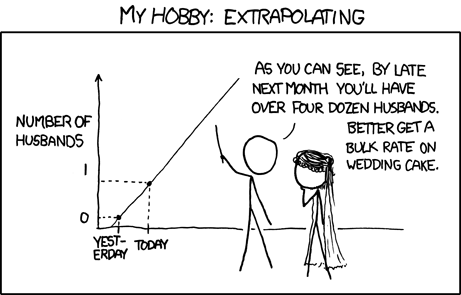
\includegraphics[width=0.75\textwidth,height=\textheight]{"images/linearprojectioncomic.png"}
\end{frame}

\begin{frame}{Estimating the CEF}
\protect\hypertarget{estimating-the-cef}{}
Let

\[
y_i=\beta_0+\beta_1x_i+\epsilon
\]

\begin{itemize}
\item
  Run a linear regression of \(y_i\) on \(x_i\)
\item
  Get estimates \(\hat{\beta}_0\) and \(\hat{\beta}_1\) of the true
  population \(\beta_0\) and \(\beta_1\)
\item
  Calculate \(\hat{y}_i=\hat{\beta}_0+\hat{\beta}_1x_i\), the predicted
  value for \(y_i\) given \(x_i\), such that \[
  \hat{y}_i=E[y_i|x_i], \text{ the CEF.}
  \] If you are interested in description or prediction, this is fine
  and we can end the class here!
\end{itemize}
\end{frame}

\begin{frame}{Application: Regression for Prediction}
\protect\hypertarget{application-regression-for-prediction}{}
Who might be interested in using regressions for prediction?

Suppose you are a bank interested in predicting customer's ability to
repay student loans. You have a subset of CPS data on earnings and the
number of years spent in education.

You estimate the following on working age adults (22+):

\[
Income_i=\beta_0+\beta_1 Schooling_i+\epsilon_i
\]
\end{frame}

\begin{frame}{Application: Lets do some coding!}
\protect\hypertarget{application-lets-do-some-coding}{}
\center 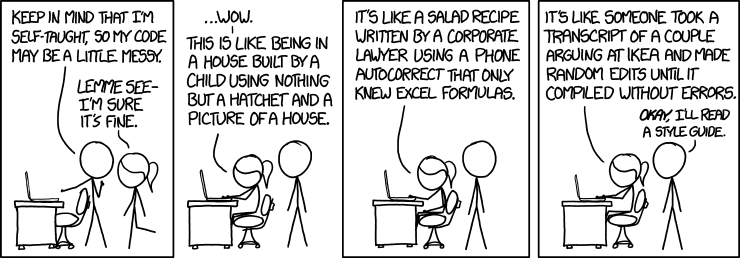
\includegraphics[width=0.75\textwidth,height=\textheight]{"images/code_quality.png"}
\end{frame}

\begin{frame}[fragile]{Application: Regression for Prediction}
\protect\hypertarget{application-regression-for-prediction-1}{}
\tiny

\begin{Shaded}
\begin{Highlighting}[]
\NormalTok{mydata\textless{}{-}}\KeywordTok{read.csv}\NormalTok{(}\StringTok{"../../data/data\_M1\_OVB/cps\_clean.csv"}\NormalTok{)}

\NormalTok{reg1\textless{}{-}}\KeywordTok{lm}\NormalTok{(inctot}\OperatorTok{\textasciitilde{}}\NormalTok{edu,mydata[mydata}\OperatorTok{$}\NormalTok{age}\OperatorTok{\textgreater{}}\DecValTok{22}\NormalTok{,])}
\KeywordTok{summary}\NormalTok{(reg1)}
\end{Highlighting}
\end{Shaded}

\begin{verbatim}
## 
## Call:
## lm(formula = inctot ~ edu, data = mydata[mydata$age > 22, ])
## 
## Residuals:
##     Min      1Q  Median      3Q     Max 
## -107200  -31055  -11015   13207 1069070 
## 
## Coefficients:
##             Estimate Std. Error t value Pr(>|t|)    
## (Intercept) -61933.9     5339.0  -11.60   <2e-16 ***
## edu           8054.0      375.3   21.46   <2e-16 ***
## ---
## Signif. codes:  0 '***' 0.001 '**' 0.01 '*' 0.05 '.' 0.1 ' ' 1
## 
## Residual standard error: 72970 on 4644 degrees of freedom
## Multiple R-squared:  0.09022,    Adjusted R-squared:  0.09003 
## F-statistic: 460.6 on 1 and 4644 DF,  p-value: < 2.2e-16
\end{verbatim}

\textbf{Interpret your results.}
\end{frame}

\begin{frame}[fragile]{Application: Regression for Prediction}
\protect\hypertarget{application-regression-for-prediction-2}{}
\tiny

\begin{Shaded}
\begin{Highlighting}[]
\KeywordTok{summary}\NormalTok{(reg1)}
\end{Highlighting}
\end{Shaded}

\begin{verbatim}
## 
## Call:
## lm(formula = inctot ~ edu, data = mydata[mydata$age > 22, ])
## 
## Residuals:
##     Min      1Q  Median      3Q     Max 
## -107200  -31055  -11015   13207 1069070 
## 
## Coefficients:
##             Estimate Std. Error t value Pr(>|t|)    
## (Intercept) -61933.9     5339.0  -11.60   <2e-16 ***
## edu           8054.0      375.3   21.46   <2e-16 ***
## ---
## Signif. codes:  0 '***' 0.001 '**' 0.01 '*' 0.05 '.' 0.1 ' ' 1
## 
## Residual standard error: 72970 on 4644 degrees of freedom
## Multiple R-squared:  0.09022,    Adjusted R-squared:  0.09003 
## F-statistic: 460.6 on 1 and 4644 DF,  p-value: < 2.2e-16
\end{verbatim}

\normalsize

So an extra year of education \textbf{predicts} earnings that are 8,054
USD higher (since \(\hat{\beta}_1=8054\)).
\end{frame}

\begin{frame}{Application: Regression for Prediction}
\protect\hypertarget{application-regression-for-prediction-3}{}
\center 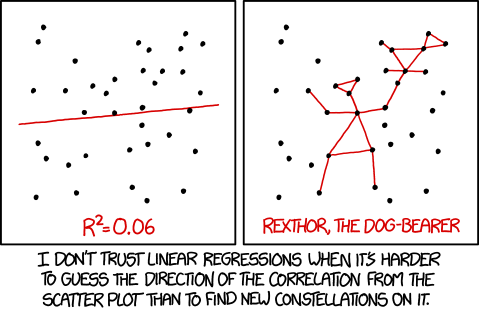
\includegraphics[width=0.75\textwidth,height=\textheight]{"images/scatterintuitioncomic.png"}
\end{frame}

\begin{frame}[fragile]{Application: Regression for Prediction}
\protect\hypertarget{application-regression-for-prediction-4}{}
\tiny

\begin{Shaded}
\begin{Highlighting}[]
\KeywordTok{plot}\NormalTok{(mydata[mydata}\OperatorTok{$}\NormalTok{age}\OperatorTok{\textgreater{}}\DecValTok{22}\NormalTok{,]}\OperatorTok{$}\NormalTok{edu, }
\NormalTok{     mydata[mydata}\OperatorTok{$}\NormalTok{age}\OperatorTok{\textgreater{}}\DecValTok{22}\NormalTok{,]}\OperatorTok{$}\NormalTok{inctot)}
\end{Highlighting}
\end{Shaded}

\includegraphics{Slides_OVB_files/figure-beamer/chunk1a-1.pdf}
\end{frame}

\begin{frame}{Application: Regression for Prediction}
\protect\hypertarget{application-regression-for-prediction-5}{}
Using these estimate we can predict the difference in annual income
between a high school and college grad as

\[\begin{aligned}
\widehat{Income}_{col}-\widehat{Income}_{hs} & =(\hat{\beta_0}+\hat{\beta_1}*16)-(\hat{\beta_0}+\hat{\beta_1}*12)\\
& =\hat{\beta_1}*4\\
& = 8,054*4=\$32,216.
\end{aligned}\]

So we would \textbf{predict} annual returns of \$32,216.
\end{frame}

\begin{frame}{Application: Regression for Prediction}
\protect\hypertarget{application-regression-for-prediction-6}{}
Alternatively, we could create an indicator variable set to 1 for
individuals with college educations and estimate it on the subset of
individuals who have at least 12 years of schooling:

\begin{equation}
\begin{split}
Income_i=\beta_0+\beta_1 CollGrad_i+\epsilon_i
\end{split}
\end{equation}
\end{frame}

\begin{frame}[fragile]{Application: Regression for Prediction}
\protect\hypertarget{application-regression-for-prediction-7}{}
\tiny

\begin{Shaded}
\begin{Highlighting}[]
\NormalTok{mydata}\OperatorTok{$}\NormalTok{collgrad\textless{}{-}}\DecValTok{0}
\NormalTok{mydata}\OperatorTok{$}\NormalTok{collgrad[mydata}\OperatorTok{$}\NormalTok{edu}\OperatorTok{\textgreater{}=}\DecValTok{16}\NormalTok{]\textless{}{-}}\DecValTok{1}

\NormalTok{reg2\textless{}{-}}\KeywordTok{lm}\NormalTok{(inctot}\OperatorTok{\textasciitilde{}}\NormalTok{collgrad,mydata[mydata}\OperatorTok{$}\NormalTok{edu}\OperatorTok{\textgreater{}=}\DecValTok{12} \OperatorTok{\&}\StringTok{ }\NormalTok{mydata}\OperatorTok{$}\NormalTok{age}\OperatorTok{\textgreater{}}\DecValTok{22}\NormalTok{,])}
\KeywordTok{summary}\NormalTok{(reg2)}
\end{Highlighting}
\end{Shaded}

\begin{verbatim}
## 
## Call:
## lm(formula = inctot ~ collgrad, data = mydata[mydata$edu >= 12 & 
##     mydata$age > 22, ])
## 
## Residuals:
##     Min      1Q  Median      3Q     Max 
##  -91324  -31425  -11433   13518 1054675 
## 
## Coefficients:
##             Estimate Std. Error t value Pr(>|t|)    
## (Intercept)    36483       1478   24.69   <2e-16 ***
## collgrad       44842       2409   18.61   <2e-16 ***
## ---
## Signif. codes:  0 '***' 0.001 '**' 0.01 '*' 0.05 '.' 0.1 ' ' 1
## 
## Residual standard error: 76010 on 4240 degrees of freedom
## Multiple R-squared:  0.07554,    Adjusted R-squared:  0.07532 
## F-statistic: 346.4 on 1 and 4240 DF,  p-value: < 2.2e-16
\end{verbatim}

\normalsize

Interpret your results.
\end{frame}

\begin{frame}[fragile]{Application: Regression for Prediction}
\protect\hypertarget{application-regression-for-prediction-8}{}
\tiny

\begin{Shaded}
\begin{Highlighting}[]
\NormalTok{mydata}\OperatorTok{$}\NormalTok{collgrad\textless{}{-}}\DecValTok{0}
\NormalTok{mydata}\OperatorTok{$}\NormalTok{collgrad[mydata}\OperatorTok{$}\NormalTok{edu}\OperatorTok{\textgreater{}=}\DecValTok{16}\NormalTok{]\textless{}{-}}\DecValTok{1}

\NormalTok{reg2\textless{}{-}}\KeywordTok{lm}\NormalTok{(inctot}\OperatorTok{\textasciitilde{}}\NormalTok{collgrad,mydata[mydata}\OperatorTok{$}\NormalTok{edu}\OperatorTok{\textgreater{}=}\DecValTok{12} \OperatorTok{\&}\StringTok{ }\NormalTok{mydata}\OperatorTok{$}\NormalTok{age}\OperatorTok{\textgreater{}}\DecValTok{22}\NormalTok{,])}
\KeywordTok{summary}\NormalTok{(reg2)}
\end{Highlighting}
\end{Shaded}

\begin{verbatim}
## 
## Call:
## lm(formula = inctot ~ collgrad, data = mydata[mydata$edu >= 12 & 
##     mydata$age > 22, ])
## 
## Residuals:
##     Min      1Q  Median      3Q     Max 
##  -91324  -31425  -11433   13518 1054675 
## 
## Coefficients:
##             Estimate Std. Error t value Pr(>|t|)    
## (Intercept)    36483       1478   24.69   <2e-16 ***
## collgrad       44842       2409   18.61   <2e-16 ***
## ---
## Signif. codes:  0 '***' 0.001 '**' 0.01 '*' 0.05 '.' 0.1 ' ' 1
## 
## Residual standard error: 76010 on 4240 degrees of freedom
## Multiple R-squared:  0.07554,    Adjusted R-squared:  0.07532 
## F-statistic: 346.4 on 1 and 4240 DF,  p-value: < 2.2e-16
\end{verbatim}

\normalsize

\(\hat{\beta}_1=44,842\), so having a four year college degree
\textbf{predicts} earnings that are \$44,842 higher.
\end{frame}

\begin{frame}{Application: Regression for Prediction}
\protect\hypertarget{application-regression-for-prediction-9}{}
The key point: we are not saying that the college degree \textbf{caused}
higher earnings, but it does \textbf{predict} higher earnings. For many
applications, prediction is enough.

To get causation, we need to do a lot more work.

\center 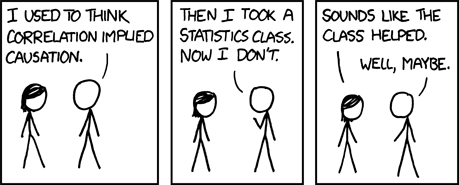
\includegraphics[width=0.75\textwidth,height=\textheight]{"images/corcauscomic.png"}
\end{frame}

\begin{frame}{``No Causation Without Manipulation''}
\protect\hypertarget{no-causation-without-manipulation}{}
\textbf{What if we are interested in causal effects?}

It was easy to estimate the relationship between income and schooling.
As illustrated in the application, I estimated

\[
Income_i=\beta_0+\beta_i Schooling_i+\epsilon 
\] and was able to recover the conditional expectation function

\[
E[Income_i|Schooling_i]=\hat{Income}_i=\hat{\beta}_0+\hat{\beta}_1Schooling_i 
\] BUT this only tells us how income and schooling co-vary. This
\textbf{DOES NOT} tell us what would happen to income if there was an
\textbf{``exogenous''} change in schooling.
\end{frame}

\begin{frame}{What is the difference?}
\protect\hypertarget{what-is-the-difference}{}
Here, schooling is \textbf{``endogenously''} determined.

\textbf{Who is most likely to select into schooling?}
\end{frame}

\begin{frame}{What is the difference?}
\protect\hypertarget{what-is-the-difference-1}{}
Here, schooling is \textbf{``endogenously''} determined. For example:

\begin{itemize}
\item
  those who expect to benefit the most select into schooling.
\item
  those with the highest family incomes select into schooling.
\end{itemize}

A regression coefficient estimated using data on \textbf{endogenous}
schooling choices will not correspond to the effects of an
\textbf{exogenous} change in schooling.

To estimate the \textbf{causal} effect, we will need to identify some
type of \textbf{manipulation} that created an \textbf{exogenous} change
in schooling.
\end{frame}

\begin{frame}{A note on interpretation}
\protect\hypertarget{a-note-on-interpretation}{}
It in NOT the case that the endogenous estimate is \textit{wrong} and
the exogenous estimate is \textit{right}. They are simply measuring
different things and should be interpreted accordingly.

Regarding our estimates using the endogenous CPS data:

\textbf{CORRECT:}

\emph{``We can expect the earnings of a person with one additional year
of schooling to be \$ \(\hat{\beta}_1\) higher.''}

\textbf{INCORRECT:}

\emph{``One additional year of schooling CAUSES earnings to increase by
\$ \(\hat{\beta}_1\).''}
\end{frame}

\begin{frame}{The Rubin Causal Model}
\protect\hypertarget{the-rubin-causal-model}{}
\textbf{\emph{Two roads diverged in a yellow wood,}}\\
\textbf{\emph{And sorry I could not travel both}}\\
\textbf{\emph{--Robert Frost}}

To understand causal inference, it is helpful to think about how a unit
has different potential outcomes depending on it's treatment status.
\end{frame}

\begin{frame}{The Rubin Causal Model}
\protect\hypertarget{the-rubin-causal-model-1}{}
Let \(D_i\) be a binary treatment variable that could affect outcome
\(Y_i\). Each unit faces two potential outcomes:

\[
\begin{split}
Y_i& = \begin{cases}
      Y_i(1) & \text{ if } D_i=1 \text{ (\textit{the treatment condition})}\\
      Y_i(0) & \text{ if } D_i=0 \text{ (\textit{the control condition})}
    \end{cases}  \\
\end{split}
\] The problem: Unobserved \textbf{counterfactuals}. We will never
observe both \(Y_i(1)\) and \(Y_i(0)\).
\end{frame}

\begin{frame}{Example: Does going to college cause higher earnings?}
\protect\hypertarget{example-does-going-to-college-cause-higher-earnings}{}
Let the treatment, \(D_i\) be going to college. Each high school
graduate faces two potential outcomes:

\[
\begin{split}
\text{\textit{potential outcomes}}= \begin{cases}
      earn_{i,col} & \text{ if \textit{i} goes to college} \text{ (\textit{treatment})}\\
      earn_{i,no col} & \text{ if \textit{i} no college} \text{ (\textit{control})}
    \end{cases}  
\end{split}
\]

We can conceive of both \(earn_{i,col}\) and \(earn_{i,no col}\) (but
will only ever observe one or the other).

The treatment is potentially manipulable: we can imagine a policy or
intervention that could make either of these values observable.
\end{frame}

\begin{frame}{``No Causation without Manipulation'' (2)}
\protect\hypertarget{no-causation-without-manipulation-2}{}
Can you conceptualize both \(Y_i(1)\) and \(Y_i(0)\) for the same unit?

\textbf{\underline{If no:}} \(D\) does not correspond to a potentially
manipulable treatment.

\begin{itemize}
\tightlist
\item
  We need to further define the problem.
\end{itemize}

\textbf{Example: Does being a woman \underline{cause} lower earnings?}
\end{frame}

\begin{frame}{``No Causation without Manipulation'' (2)}
\protect\hypertarget{no-causation-without-manipulation-2-1}{}
Can you conceptualize both \(Y_i(1)\) and \(Y_i(0)\) for the same unit?

\textbf{\underline{If no:}} \(D\) does not correspond to a potentially
manipulable treatment.

\begin{itemize}
\tightlist
\item
  We need to further define the problem.
\end{itemize}

\textbf{Example: Does being a woman \underline{cause} lower earnings?}

It is not possible for me to imagine some intervention that would reveal
what my earnings outcome would have been if I was a man.

We know that being a woman \textbf{\emph{predicts}} lower earnings, but
the causal question as posed is ill defined.
\end{frame}

\begin{frame}{Causal Effects}
\protect\hypertarget{causal-effects}{}
Define the causal effect of treatment \(D=1\) on outcome \(Y\) for unit
\(i\) as

\[
Y_i(1)-Y_i(0)=\tau_i
\] Note: the treatment effect is relative and specific to observation
\(i\).

But how can we identify \(\tau_i\) if we never observe both \(Y_i(1)\)
and \(Y_i(0)\) for a given unit?
\end{frame}

\begin{frame}{The Fundamental Problem of Causal Inference}
\protect\hypertarget{the-fundamental-problem-of-causal-inference}{}
It is impossible to observe the value of \(Y_i(1)\) and \(Y_i(0)\) in
the same unit \(i\) and, therefore, it is impossible to observe
\(\tau_i\), the effect for unit \(i\) of the treatment on it's outcome,
\(Y_i\). (Holland 1986)

\centering

\textbf{So, are we doomed?}
\end{frame}

\begin{frame}{The Fundamental Problem of Causal Inference}
\protect\hypertarget{the-fundamental-problem-of-causal-inference-1}{}
It is impossible to observe the value of \(Y_i(1)\) and \(Y_i(0)\) in
the same unit \(i\) and, therefore, it is impossible to observe
\(\tau_i\), the effect for unit \(i\) of the treatment on it's outcome,
\(Y_i\). (Holland 1986)

\centering

\textbf{So, are we doomed?}

\raggedright

No! Though we can't identify \(\tau_i\) at the unit level, we can
identify the \emph{Average Causal Treatment Effect} (ATE)

\[
\bar{\tau}=E[Y_i(1)-Y_i(0)]=E[Y_i(1)]-E[Y_i(0)]
\]

with the right research design, we can recover \(\bar{\tau}\).
\end{frame}

\begin{frame}{The Conditional Independence Assumption}
\protect\hypertarget{the-conditional-independence-assumption}{}
Suppose a constant treatment effect such that \(\tau=Y_i(1)-Y_i(0)\).
Since

\[
\begin{aligned}
Y_i&=Y_i(0)+(Y_i(1)-Y_i(0))D_i\\
&=Y_i(0)+\tau D_i\\
&=E[Y_i(0)]+\tau D_i+Y_i(0)-E[Y_i(0)]\\
&=\alpha+\tau D_i+\eta_i
\end{aligned}
\] where \(\alpha=E[Y_i(0)]\), \(\tau=Y_i(1)-Y_i(0)\) and \(\eta_i\) is
the random part of \(Y_i(0)\) since \(\eta_i=Y_i(0)-E[Y_i(0)]\).
\end{frame}

\begin{frame}{The Conditional Independence Assumption}
\protect\hypertarget{the-conditional-independence-assumption-1}{}
The expected outcomes of someone with and someone without treatment is
then given by

\[
\begin{aligned}
E[Y_i(1)]&=\alpha+\tau+E[\eta_i|D_i=1]\\
E[Y_i(0)]&=\alpha+E[\eta_i|D_i=0]
\end{aligned}
\]

so that the difference between these outcomes can be broken down into

\[
 E[Y_i(1)]-E[Y_i(0)] = 
    \underbrace{\tau}_\text{treatment effect} + \underbrace{E[\eta_i|D_i=1]-E[\eta_i|D_i=0]}_\text{?}
\]

What is the second term? \(\Rightarrow\) Top Hat
\end{frame}

\begin{frame}{The Conditional Independence Assumption}
\protect\hypertarget{the-conditional-independence-assumption-2}{}
The expected outcomes of someone with and someone without treatment is
then given by

\[
\begin{aligned}
E[Y_i(1)]&=\alpha+\tau+E[\eta_i|D_i=1]\\
E[Y_i(0)]&=\alpha+E[\eta_i|D_i=0]
\end{aligned}
\]

so that the difference between these outcomes can be broken down into

\[
 E[Y_i(1)]-E[Y_i(0)] = 
    \underbrace{\tau}_\text{treatment effect} + \underbrace{E[\eta_i|D_i=1]-E[\eta_i|D_i=0]}_\text{selection bias}
\]
\end{frame}

\begin{frame}{The Conditional Independence Assumption}
\protect\hypertarget{the-conditional-independence-assumption-3}{}
So if I run \(Y_i=\alpha+\tau D_i+\eta_i\), the estimated
\(\tilde{\tau}\neq \tau\) if there is selection bias such that
\(E[\eta_i|D_i=1]\neq E[\eta_i|D_i=0]\).

This will occur if absent treatment, those who would select into
treatment have a different expected outcome compared to those who would
not select into treatment \[
E[Y_i(0)|D_i=1]\neq E[Y_i(0)|D_i=0],
\] because treatment is not random. Formally,

\[
\{Y_i(1), Y_i(0)\} \not\perp  D_i.
\]
\end{frame}

\begin{frame}{Example}
\protect\hypertarget{example}{}
I naively use my observational CPS data and estimate \[
\begin{split}
earnings_i=\tilde{\alpha}+\tilde{\tau} college_i+\epsilon_i.
\end{split}
\] If I want to estimate \(\tau\), the \textbf{causal} effect of a
college degree on earnings, this estimate, \(\tilde{\tau}\) will be
biased: \(E[\tilde{\tau}]\neq \tau\).

Why?
\end{frame}

\begin{frame}{Example}
\protect\hypertarget{example-1}{}
I naively use my observational CPS data and estimate \[
\begin{split}
earnings_i=\tilde{\alpha}+\tilde{\tau} college_i+\epsilon_i.
\end{split}
\] If I want to estimate \(\tau\), the \textbf{causal} effect of a
college degree on earnings, this estimate, \(\tilde{\tau}\) will be
biased: \(E[\tilde{\tau}]\neq \tau\).

Why?

\underline{Selection bias:} If people who receive college degrees would
have had higher earnings even without the degree,

\[
E[\eta_i|D_i=1]>E[\eta_i|D_i=0].
\]
\end{frame}

\begin{frame}{The Conditional Independence Assumption}
\protect\hypertarget{the-conditional-independence-assumption-4}{}
\textbf{The Conditional Independence Assumption}: conditional on
observed characteristics, \(X_i\), selection bias disappears and \[
\{Y_i(1), Y_i(0)\} \perp  D_i|X_i.
\]

If CIA holds, once I control for \(X_i\), treatment is as good as
randomly assigned. If this is the case, our comparisons have a causal
interpretation and

\[
E[Y_i(1)|X_i]-E[Y_i(0)|X_i]=E[Y_i(1)-Y_i(0)|X_i].
\]
\end{frame}

\begin{frame}{The Conditional Independence Assumption}
\protect\hypertarget{the-conditional-independence-assumption-5}{}
\center 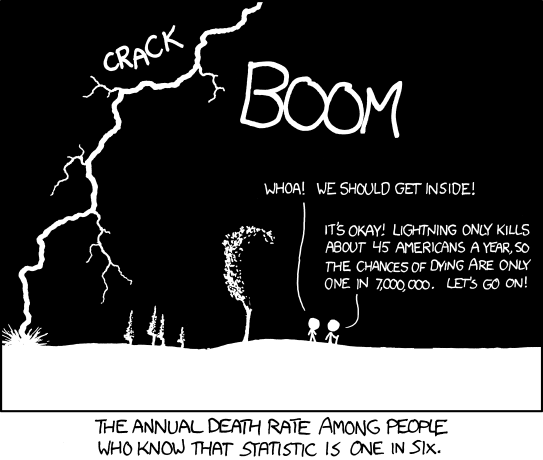
\includegraphics[width=0.5\textwidth,height=\textheight]{"images/ciacomic.png"}
\end{frame}

\begin{frame}{CIA in Regressions}
\protect\hypertarget{cia-in-regressions}{}
If I estimate \(Y_i=\alpha+\tau D_i +\eta_i\),
\(E[\tilde{\tau}]\neq \tau\) due to selection bias. \textbf{Now suppose
CIA holds given a vector of observed covariates, \(X'_i\).}

\begin{itemize}
\item
  I can decompose \(\eta_i\): \(\eta_i=X'_i\gamma+\nu_i\) with:
  \(E[\eta_i|X_i]=X'_i\gamma\)
\item
  If the CIA assumption holds, then \[
  E[Y_i(D)|X_i]=\alpha+\tau D_i+X'_i \gamma
  \] and \[
  Y_i(D)=\alpha+\tau D_i+X'_i \gamma+\nu_i
  \] where the \(\nu_i\) residuals are uncorrelated with \(D_i\) and
  \(X'_i\).
\item
  Thus \[
  E[\hat{\tau}]=\tau
  \] and we can interpret \(\hat{\tau}\) as the causal effect of
  interest.
\end{itemize}
\end{frame}

\begin{frame}{Example:}
\protect\hypertarget{example-2}{}
If I estimate
\(Earnings_i=\tilde{\alpha}+\tilde{\tau}college_i+\epsilon_i\) we saw
that \(E[\tilde{\tau}]\neq\tau\) due to selection bias.

\textbf{Suppose CIA holds if I condition on a student's household
income.} (ie. if I control for student household income, which students
complete college is as good as randomly assigned) .

Then \[
earnings_i=\hat{\alpha}+\hat{\tau}college_i+\hat{\gamma}hhinc_i+\epsilon_i
\] and \(E[\hat{\tau}]=\tau\): a college degree causes earnings to
increase by \(\hat{\tau}\) USD.

\textbf{WARNING: This is a big assumption, that often does not hold.}
\end{frame}

\begin{frame}{Omitted Variable Bias}
\protect\hypertarget{omitted-variable-bias}{}
Suppose the true model is given by \[
Y_i=\beta_0+\beta_1 x_{1i}+\beta_2 x_{2i}+\nu_i
\] but I failed to include \(x_{2i}\) and instead estimated \[
Y_i=\tilde{\beta}_0+\tilde{\beta}_1 x_{1i}+\epsilon_i.
\] If there is a relationship between \(x_{1i}\) and \(x_{2i}\) such
that \[
x_{2i}=\rho_0+\rho_1 x_{1i}+\varepsilon_i
\] we can substitute this into the first equation and by rearranging, \[
Y_i=\underbrace{(\beta_0+\beta_2\rho_0)}_{\tilde{\beta}_0}+\underbrace{(\beta_1+\beta_2 \rho_2)}_{\tilde{\beta}_1} x_{1i}+\underbrace{(\beta_2 \varepsilon_i+\nu_i)}_{\epsilon_i},
\] show that \[
\tilde{\beta_1}=\underbrace{\beta_1}_\text{treatment effect}+\underbrace{\beta_2 \rho_2}_\text{bias}.
\]
\end{frame}

\begin{frame}{Omitted variable bias}
\protect\hypertarget{omitted-variable-bias-1}{}
\[
\tilde{\beta_1}-\beta_1=\underbrace{\beta_2 \rho_2}_\text{bias}
\]

We can thus sign the bias by signing \(\beta_2\), the covariance between
\(x_{2i}\) and \(Y_i\), and signing \(\rho_2\), the covariance between
\(x_{2i}\) and \(x_{1i}\).

\begin{longtable}[]{@{}lll@{}}
\toprule
-------------------- & \(Cov(x,x_{ov})>0\) &
\(Cov(x,x_{ov})<0\)\tabularnewline
\midrule
\endhead
\(Cov(y,x_{ov})>0\) & Upward Bias & Downward Bias\tabularnewline
\(Cov(y,x_{ov})<0\) & Downward Bias & Upward Bias\tabularnewline
\bottomrule
\end{longtable}
\end{frame}

\begin{frame}{Example: Using CPS data}
\protect\hypertarget{example-using-cps-data}{}
I am interested in how health relates to income. Using my CPS sample of
working age adults I estimate \[
Income_i=\beta_0+\beta_1Health_i+\epsilon, 
\] where heath is a respondents subjective assessment of their health
with 1 being very healthy and 5 being very unhealthy.
\end{frame}

\begin{frame}[fragile]{Example: Using CPS data}
\protect\hypertarget{example-using-cps-data-1}{}
\tiny

\begin{Shaded}
\begin{Highlighting}[]
\NormalTok{reghealth\textless{}{-}}\KeywordTok{lm}\NormalTok{(inctot}\OperatorTok{\textasciitilde{}}\NormalTok{health,mydata)}
\KeywordTok{summary}\NormalTok{(reghealth)}
\end{Highlighting}
\end{Shaded}

\begin{verbatim}
## 
## Call:
## lm(formula = inctot ~ health, data = mydata)
## 
## Residuals:
##     Min      1Q  Median      3Q     Max 
##  -59413  -32893  -15716   11198 1103107 
## 
## Coefficients:
##             Estimate Std. Error t value Pr(>|t|)    
## (Intercept)  65599.6     2414.9  27.164   <2e-16 ***
## health       -8176.8      991.9  -8.243   <2e-16 ***
## ---
## Signif. codes:  0 '***' 0.001 '**' 0.01 '*' 0.05 '.' 0.1 ' ' 1
## 
## Residual standard error: 73960 on 4998 degrees of freedom
## Multiple R-squared:  0.01341,    Adjusted R-squared:  0.01322 
## F-statistic: 67.95 on 1 and 4998 DF,  p-value: < 2.2e-16
\end{verbatim}

\normalsize

Interpret.
\end{frame}

\begin{frame}{Example: Using CPS data}
\protect\hypertarget{example-using-cps-data-2}{}
How might the omission of age be biasing these estimates?

\(\Rightarrow\) Top Hat
\end{frame}

\begin{frame}{Example: Using CPS data}
\protect\hypertarget{example-using-cps-data-3}{}
How might the omission of age be biasing these estimates?

\begin{itemize}
\item
  \(cov(health_i,age_i)>0\)
\item
  \(cov(income_i,age_i)>0\)
\item
  \(\Rightarrow\) upward bias.
\end{itemize}
\end{frame}

\begin{frame}[fragile]{Example: Using CPS data}
\protect\hypertarget{example-using-cps-data-4}{}
\tiny

\begin{Shaded}
\begin{Highlighting}[]
\NormalTok{reghealth2\textless{}{-}}\KeywordTok{lm}\NormalTok{(inctot}\OperatorTok{\textasciitilde{}}\NormalTok{health}\OperatorTok{+}\NormalTok{age ,mydata)}
\KeywordTok{summary}\NormalTok{(reghealth2)}
\end{Highlighting}
\end{Shaded}

\begin{verbatim}
## 
## Call:
## lm(formula = inctot ~ health + age, data = mydata)
## 
## Residuals:
##     Min      1Q  Median      3Q     Max 
##  -84573  -31695  -12625   11680 1101885 
## 
## Coefficients:
##             Estimate Std. Error t value Pr(>|t|)    
## (Intercept)    28903       3771   7.665 2.13e-14 ***
## health        -11489       1012 -11.355  < 2e-16 ***
## age             1066         85  12.541  < 2e-16 ***
## ---
## Signif. codes:  0 '***' 0.001 '**' 0.01 '*' 0.05 '.' 0.1 ' ' 1
## 
## Residual standard error: 72830 on 4997 degrees of freedom
## Multiple R-squared:  0.04352,    Adjusted R-squared:  0.04314 
## F-statistic: 113.7 on 2 and 4997 DF,  p-value: < 2.2e-16
\end{verbatim}

\normalsize
\end{frame}

\begin{frame}{Example: Using CPS data}
\protect\hypertarget{example-using-cps-data-5}{}
How might the omission of schooling be biasing these estimates?

\(\Rightarrow\) Top Hat
\end{frame}

\begin{frame}{Example: Using CPS data}
\protect\hypertarget{example-using-cps-data-6}{}
How might the omission of schooling be biasing these estimates?

\begin{itemize}
\item
  \(cov(health_i,schooling_i)<0\)
\item
  \(cov(income_i,schooling_i)>0\)
\item
  \(\Rightarrow\) downward bias.
\end{itemize}
\end{frame}

\begin{frame}[fragile]{Example: Using CPS data}
\protect\hypertarget{example-using-cps-data-7}{}
\tiny

\begin{Shaded}
\begin{Highlighting}[]
\NormalTok{reghealth3\textless{}{-}}\KeywordTok{lm}\NormalTok{(inctot}\OperatorTok{\textasciitilde{}}\NormalTok{health}\OperatorTok{+}\NormalTok{age}\OperatorTok{+}\NormalTok{edu ,mydata)}
\KeywordTok{summary}\NormalTok{(reghealth3)}
\end{Highlighting}
\end{Shaded}

\begin{verbatim}
## 
## Call:
## lm(formula = inctot ~ health + age + edu, data = mydata)
## 
## Residuals:
##     Min      1Q  Median      3Q     Max 
## -117272  -28392   -9807   12671 1077286 
## 
## Coefficients:
##              Estimate Std. Error t value Pr(>|t|)    
## (Intercept) -82442.91    6501.39 -12.681  < 2e-16 ***
## health       -6315.25    1003.36  -6.294 3.36e-10 ***
## age            953.42      81.79  11.657  < 2e-16 ***
## edu           7540.90     365.73  20.619  < 2e-16 ***
## ---
## Signif. codes:  0 '***' 0.001 '**' 0.01 '*' 0.05 '.' 0.1 ' ' 1
## 
## Residual standard error: 69920 on 4996 degrees of freedom
## Multiple R-squared:  0.1185, Adjusted R-squared:  0.118 
## F-statistic: 223.9 on 3 and 4996 DF,  p-value: < 2.2e-16
\end{verbatim}

\normalsize
\end{frame}

\begin{frame}[fragile]{Example: Presenting results}
\protect\hypertarget{example-presenting-results}{}
\tiny

\begin{Shaded}
\begin{Highlighting}[]
\KeywordTok{stargazer}\NormalTok{(reghealth,reghealth2, reghealth3, }\DataTypeTok{type=}\StringTok{"latex"}\NormalTok{, }\DataTypeTok{header=}\OtherTok{FALSE}\NormalTok{, }
          \DataTypeTok{title=}\StringTok{"Income and health"}\NormalTok{, }\DataTypeTok{omit.stat=}\KeywordTok{c}\NormalTok{(}\StringTok{"f"}\NormalTok{, }\StringTok{"ser"}\NormalTok{))}
\end{Highlighting}
\end{Shaded}

\begin{table}[!htbp] \centering 
  \caption{Income and health} 
  \label{} 
\begin{tabular}{@{\extracolsep{5pt}}lccc} 
\\[-1.8ex]\hline 
\hline \\[-1.8ex] 
 & \multicolumn{3}{c}{\textit{Dependent variable:}} \\ 
\cline{2-4} 
\\[-1.8ex] & \multicolumn{3}{c}{inctot} \\ 
\\[-1.8ex] & (1) & (2) & (3)\\ 
\hline \\[-1.8ex] 
 health & $-$8,176.764$^{***}$ & $-$11,489.250$^{***}$ & $-$6,315.248$^{***}$ \\ 
  & (991.929) & (1,011.858) & (1,003.357) \\ 
  & & & \\ 
 age &  & 1,066.011$^{***}$ & 953.415$^{***}$ \\ 
  &  & (85.002) & (81.792) \\ 
  & & & \\ 
 edu &  &  & 7,540.903$^{***}$ \\ 
  &  &  & (365.735) \\ 
  & & & \\ 
 Constant & 65,599.570$^{***}$ & 28,903.240$^{***}$ & $-$82,442.910$^{***}$ \\ 
  & (2,414.934) & (3,770.567) & (6,501.394) \\ 
  & & & \\ 
\hline \\[-1.8ex] 
Observations & 5,000 & 5,000 & 5,000 \\ 
R$^{2}$ & 0.013 & 0.044 & 0.119 \\ 
Adjusted R$^{2}$ & 0.013 & 0.043 & 0.118 \\ 
\hline 
\hline \\[-1.8ex] 
\textit{Note:}  & \multicolumn{3}{r}{$^{*}$p$<$0.1; $^{**}$p$<$0.05; $^{***}$p$<$0.01} \\ 
\end{tabular} 
\end{table} 
\normalsize

Check out jakeruss.com/cheatsheets/stargazer/
\end{frame}

\begin{frame}{Example: Using CPS data}
\protect\hypertarget{example-using-cps-data-8}{}
So is our estimate of \(\beta_1\) in column 3 the causal effect of
health on income?

Does the CIA hold?

Conditional on age and schooling, is subjective health as good as
randomly assigned?
\end{frame}

\begin{frame}[fragile]{Building intuition: A simulation}
\protect\hypertarget{building-intuition-a-simulation}{}
Suppose the data generating process (DGP) is as follows: my outcome
variable, \(Y\) depends on two variables, \(V_1\) and \(V_2\) such that

\[
Y_i=\beta_0+\beta_1 V_{1i}+\beta_2 V_{2i}+\epsilon_i
\]

where \(V_1\) and \(V_2\) are correlated with \(Cor(V_1,V_2)=0.5\).

\tiny

\begin{Shaded}
\begin{Highlighting}[]
\KeywordTok{library}\NormalTok{(MASS)}
\KeywordTok{library}\NormalTok{(ggplot2)}
\end{Highlighting}
\end{Shaded}

\begin{verbatim}
## Warning: package 'ggplot2' was built under R version 3.6.2
\end{verbatim}

\begin{Shaded}
\begin{Highlighting}[]
\KeywordTok{set.seed}\NormalTok{(}\DecValTok{1999}\NormalTok{)}
\NormalTok{out \textless{}{-}}\StringTok{ }\KeywordTok{as.data.frame}\NormalTok{(}\KeywordTok{mvrnorm}\NormalTok{(}\DecValTok{1000}\NormalTok{, }\DataTypeTok{mu =} \KeywordTok{c}\NormalTok{(}\DecValTok{0}\NormalTok{,}\DecValTok{0}\NormalTok{), }
                     \DataTypeTok{Sigma =} \KeywordTok{matrix}\NormalTok{(}\KeywordTok{c}\NormalTok{(}\DecValTok{1}\NormalTok{,}\FloatTok{0.5}\NormalTok{,}\FloatTok{0.5}\NormalTok{,}\DecValTok{1}\NormalTok{), }\DataTypeTok{ncol =} \DecValTok{2}\NormalTok{), }
                     \DataTypeTok{empirical =} \OtherTok{TRUE}\NormalTok{))}
\KeywordTok{cor}\NormalTok{(out)}
\end{Highlighting}
\end{Shaded}

\begin{verbatim}
##     V1  V2
## V1 1.0 0.5
## V2 0.5 1.0
\end{verbatim}

\normalsize
\end{frame}

\begin{frame}[fragile]{Building intuition: A simulation}
\protect\hypertarget{building-intuition-a-simulation-1}{}
\begin{Shaded}
\begin{Highlighting}[]
\KeywordTok{plot}\NormalTok{(out)}
\end{Highlighting}
\end{Shaded}

\includegraphics{Slides_OVB_files/figure-beamer/sim1a-1.pdf}
\end{frame}

\begin{frame}[fragile]{Building intuition: A simulation}
\protect\hypertarget{building-intuition-a-simulation-2}{}
I add an error term for each observation and then simulate the true DGP
with \(\beta_1=5\) and \(\beta_2=7\).

\tiny

\begin{Shaded}
\begin{Highlighting}[]
\NormalTok{out}\OperatorTok{$}\NormalTok{error\textless{}{-}}\KeywordTok{rnorm}\NormalTok{(}\DecValTok{1000}\NormalTok{, }\DataTypeTok{mean=}\DecValTok{0}\NormalTok{, }\DataTypeTok{sd=}\DecValTok{1}\NormalTok{)}

\NormalTok{B1\textless{}{-}}\DecValTok{5}
\NormalTok{B2\textless{}{-}}\DecValTok{7}

\NormalTok{out}\OperatorTok{$}\NormalTok{Y\textless{}{-}out}\OperatorTok{$}\NormalTok{V1}\OperatorTok{*}\NormalTok{B1}\OperatorTok{+}\NormalTok{out}\OperatorTok{$}\NormalTok{V2}\OperatorTok{*}\NormalTok{B2}\OperatorTok{+}\NormalTok{out}\OperatorTok{$}\NormalTok{error}
\end{Highlighting}
\end{Shaded}

\normalsize

I can now estimate the correct model and an under-specified model:

\tiny

\begin{Shaded}
\begin{Highlighting}[]
\NormalTok{sim1\textless{}{-}}\KeywordTok{lm}\NormalTok{(Y}\OperatorTok{\textasciitilde{}}\NormalTok{V1}\OperatorTok{+}\NormalTok{V2, }\DataTypeTok{data=}\NormalTok{out)}

\NormalTok{sim2\textless{}{-}}\KeywordTok{lm}\NormalTok{(Y}\OperatorTok{\textasciitilde{}}\NormalTok{V1, }\DataTypeTok{data=}\NormalTok{out)}
\end{Highlighting}
\end{Shaded}

\normalsize
\end{frame}

\begin{frame}[fragile]{Building intuition: A simulation}
\protect\hypertarget{building-intuition-a-simulation-3}{}
\tiny

\begin{Shaded}
\begin{Highlighting}[]
\KeywordTok{stargazer}\NormalTok{(sim1,sim2, }\DataTypeTok{type=}\StringTok{"latex"}\NormalTok{, }\DataTypeTok{header=}\OtherTok{FALSE}\NormalTok{, }
          \DataTypeTok{title=}\StringTok{"Omitted Variable Bias Simulation"}\NormalTok{, }\DataTypeTok{omit.stat=}\KeywordTok{c}\NormalTok{(}\StringTok{"f"}\NormalTok{, }\StringTok{"ser"}\NormalTok{))}
\end{Highlighting}
\end{Shaded}

\begin{table}[!htbp] \centering 
  \caption{Omitted Variable Bias Simulation} 
  \label{} 
\begin{tabular}{@{\extracolsep{5pt}}lcc} 
\\[-1.8ex]\hline 
\hline \\[-1.8ex] 
 & \multicolumn{2}{c}{\textit{Dependent variable:}} \\ 
\cline{2-3} 
\\[-1.8ex] & \multicolumn{2}{c}{Y} \\ 
\\[-1.8ex] & (1) & (2)\\ 
\hline \\[-1.8ex] 
 V1 & 5.007$^{***}$ & 8.519$^{***}$ \\ 
  & (0.036) & (0.195) \\ 
  & & \\ 
 V2 & 7.023$^{***}$ &  \\ 
  & (0.036) &  \\ 
  & & \\ 
 Constant & $-$0.015 & $-$0.015 \\ 
  & (0.031) & (0.195) \\ 
  & & \\ 
\hline \\[-1.8ex] 
Observations & 1,000 & 1,000 \\ 
R$^{2}$ & 0.991 & 0.657 \\ 
Adjusted R$^{2}$ & 0.991 & 0.656 \\ 
\hline 
\hline \\[-1.8ex] 
\textit{Note:}  & \multicolumn{2}{r}{$^{*}$p$<$0.1; $^{**}$p$<$0.05; $^{***}$p$<$0.01} \\ 
\end{tabular} 
\end{table} 
\normalsize

\(\tilde{\beta}_1\) is upward biased since \(Cor(V_1,V_2)>0\) and
\(Cor(Y,V_2)>0\).
\end{frame}

\begin{frame}[fragile]{Building intuition: A simulation}
\protect\hypertarget{building-intuition-a-simulation-4}{}
What is adding the \(V_2\) control doing? How does it change the \(V_1\)
coefficient?

\begin{itemize}
\item
  Adding \(V_2\) in the regression removes the variation in the outcome
  variable that is explained by that control variable.
\item
  The estimates can now be based on the variation due to the explanatory
  variable you are actually interested in.
\end{itemize}

To see this, I generate \(adjY\) that ``corrects'' \(Y\) by removing the
variation in \(Y\) that is explained by \(V_2\). (I can do this since I
know the true \(\beta_2\).)

\begin{Shaded}
\begin{Highlighting}[]
\NormalTok{out}\OperatorTok{$}\NormalTok{adjY\textless{}{-}out}\OperatorTok{$}\NormalTok{Y}\OperatorTok{{-}}\NormalTok{B2}\OperatorTok{*}\NormalTok{out}\OperatorTok{$}\NormalTok{V2}
\end{Highlighting}
\end{Shaded}
\end{frame}

\begin{frame}[fragile]{Building intuition: A simulation}
\protect\hypertarget{building-intuition-a-simulation-5}{}
\tiny

\begin{Shaded}
\begin{Highlighting}[]
\NormalTok{sim3\textless{}{-}}\KeywordTok{lm}\NormalTok{(adjY}\OperatorTok{\textasciitilde{}}\NormalTok{V1, }\DataTypeTok{data=}\NormalTok{out)}

\KeywordTok{stargazer}\NormalTok{(sim1,sim2,sim3, }\DataTypeTok{type=}\StringTok{"latex"}\NormalTok{, }\DataTypeTok{header=}\OtherTok{FALSE}\NormalTok{, }
          \DataTypeTok{title=}\StringTok{"Omitted Variable Bias Simulation 2"}\NormalTok{, }\DataTypeTok{omit.stat=}\KeywordTok{c}\NormalTok{(}\StringTok{"f"}\NormalTok{, }\StringTok{"ser"}\NormalTok{))}
\end{Highlighting}
\end{Shaded}

\begin{table}[!htbp] \centering 
  \caption{Omitted Variable Bias Simulation 2} 
  \label{} 
\begin{tabular}{@{\extracolsep{5pt}}lccc} 
\\[-1.8ex]\hline 
\hline \\[-1.8ex] 
 & \multicolumn{3}{c}{\textit{Dependent variable:}} \\ 
\cline{2-4} 
\\[-1.8ex] & \multicolumn{2}{c}{Y} & adjY \\ 
\\[-1.8ex] & (1) & (2) & (3)\\ 
\hline \\[-1.8ex] 
 V1 & 5.007$^{***}$ & 8.519$^{***}$ & 5.019$^{***}$ \\ 
  & (0.036) & (0.195) & (0.031) \\ 
  & & & \\ 
 V2 & 7.023$^{***}$ &  &  \\ 
  & (0.036) &  &  \\ 
  & & & \\ 
 Constant & $-$0.015 & $-$0.015 & $-$0.015 \\ 
  & (0.031) & (0.195) & (0.031) \\ 
  & & & \\ 
\hline \\[-1.8ex] 
Observations & 1,000 & 1,000 & 1,000 \\ 
R$^{2}$ & 0.991 & 0.657 & 0.963 \\ 
Adjusted R$^{2}$ & 0.991 & 0.656 & 0.963 \\ 
\hline 
\hline \\[-1.8ex] 
\textit{Note:}  & \multicolumn{3}{r}{$^{*}$p$<$0.1; $^{**}$p$<$0.05; $^{***}$p$<$0.01} \\ 
\end{tabular} 
\end{table} 
\normalsize
\end{frame}

\begin{frame}[fragile]{Building intuition: A simulation}
\protect\hypertarget{building-intuition-a-simulation-6}{}
\tiny

\begin{Shaded}
\begin{Highlighting}[]
\NormalTok{plotted\textless{}{-}}\KeywordTok{ggplot}\NormalTok{(out, }\KeywordTok{aes}\NormalTok{(V1, }\DataTypeTok{y =}\NormalTok{ value, }\DataTypeTok{color =}\NormalTok{ variable)) }\OperatorTok{+}\StringTok{ }
\StringTok{    }\KeywordTok{geom\_point}\NormalTok{(}\KeywordTok{aes}\NormalTok{(}\DataTypeTok{y =}\NormalTok{ Y, }\DataTypeTok{col =} \StringTok{"Y"}\NormalTok{)) }\OperatorTok{+}\StringTok{ }
\StringTok{    }\KeywordTok{geom\_point}\NormalTok{(}\KeywordTok{aes}\NormalTok{(}\DataTypeTok{y =}\NormalTok{ adjY, }\DataTypeTok{col =} \StringTok{"adjY"}\NormalTok{))}\OperatorTok{+}
\StringTok{    }\KeywordTok{geom\_smooth}\NormalTok{(}\DataTypeTok{method=}\StringTok{\textquotesingle{}lm\textquotesingle{}}\NormalTok{, }\KeywordTok{aes}\NormalTok{(}\DataTypeTok{y =}\NormalTok{ Y, }\DataTypeTok{col =} \StringTok{"Y"}\NormalTok{))}\OperatorTok{+}
\StringTok{    }\KeywordTok{geom\_smooth}\NormalTok{(}\DataTypeTok{method=}\StringTok{\textquotesingle{}lm\textquotesingle{}}\NormalTok{, }\KeywordTok{aes}\NormalTok{(}\DataTypeTok{y =}\NormalTok{ adjY, }\DataTypeTok{col =} \StringTok{"adjY"}\NormalTok{))}

\NormalTok{plotted}
\end{Highlighting}
\end{Shaded}

\includegraphics{Slides_OVB_files/figure-beamer/key 4-1.pdf}

\normalsize
\end{frame}

\begin{frame}{The kitchen sink}
\protect\hypertarget{the-kitchen-sink}{}
Adding more controls is not always better.

\begin{itemize}
\item
  Irrelevant variables
\item
  Bad controls
\end{itemize}

Moreover, without a carefully thought out research design, omitted
variable bias will still be a problem.
\end{frame}

\begin{frame}{Caveat: Including irrelevant variables}
\protect\hypertarget{caveat-including-irrelevant-variables}{}
Suppose I estimate \[
\tilde y=\tilde \beta_0 + \tilde \beta_1x_1 + \tilde\beta_2x_2
\] even though the true model is actually

\[
E[y|x_1]=\beta_0+\beta_1x_1
\]

\begin{itemize}
\item
  Including \(x_2\) will not bias our estimation:
  \(E[\tilde{\beta_1}]= \beta_1\).
\item
  The variance of our estimator will be less precise:
  \(Var(\tilde{\beta_1})\geq Var(\hat{\beta_1})\).
\end{itemize}
\end{frame}

\begin{frame}{Caveat: Including irrelevant variables}
\protect\hypertarget{caveat-including-irrelevant-variables-1}{}
\center 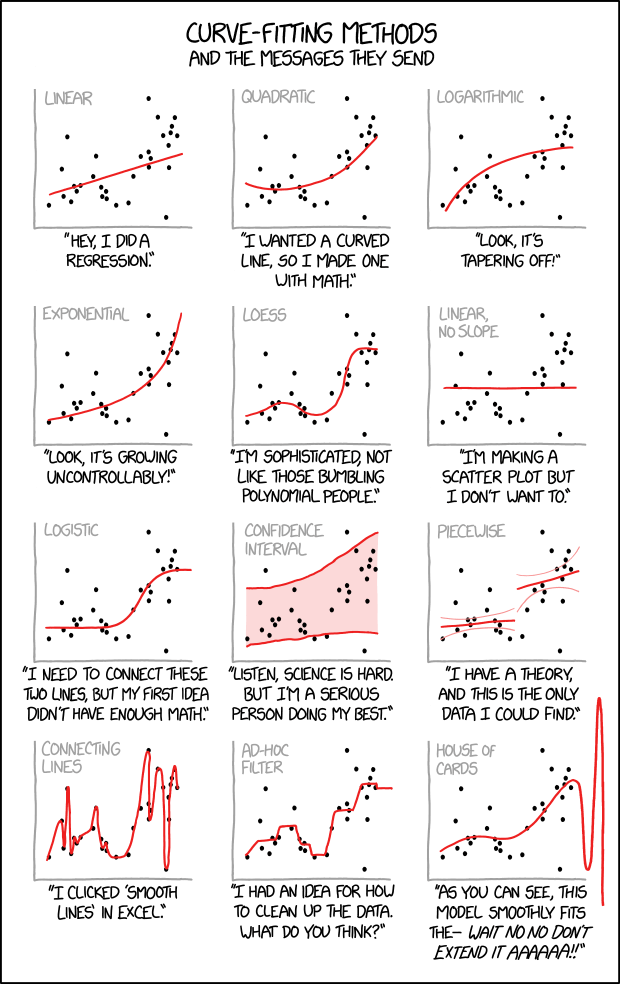
\includegraphics[width=0.45\textwidth,height=\textheight]{"images/curvefittingcomic.png"}
\end{frame}

\begin{frame}{Caveat: Bad Controls}
\protect\hypertarget{caveat-bad-controls}{}
Some control variables could themselves be outcomes of the treatment you
are evaluating.

Good controls are variables that were fixed at the time treatment was
determined.
\end{frame}

\begin{frame}{Bad Controls: Example}
\protect\hypertarget{bad-controls-example}{}
You are interested in smoking's effect on birth-weight. You estimate \[
Brthwgt_i=\beta_0+\beta_1cigday_i+\epsilon
\] but are concerned there may be important omitted variables.

You data includes information on the following: the mother's age, the
mother's education level, the number of previous pregnancies, the number
of prenatal doctor visits, mother's weight gain during pregnancy, and
alcohol use during pregnancy.

Which of these control variables should you consider adding to your
specification?

\(\Rightarrow\) Top Hat
\end{frame}

\begin{frame}{How far do controls get us?}
\protect\hypertarget{how-far-do-controls-get-us}{}
The key (untestable) assumption is that you have controlled for
everything that matters.

You are assuming that treatment assignment is ``as good as randomly
assigned''- after you have conditioned on the controls.

You are assuming that if there is any systematic selection into
``treatment'', it only depends on the observable variables you are
controlling for.

\textbf{These are VERY STRONG assumptions (that often do not hold).}
\end{frame}

\begin{frame}{There is no Santa Claus: Arseneaux, Gerber and Green
(2006)}
\protect\hypertarget{there-is-no-santa-claus-arseneaux-gerber-and-green-2006}{}
Evaluate a ``Get out the Vote'' mobilization:

\begin{itemize}
\item
  Who gets called (\(Call_i\)) is random
\item
  Who answers the call (\(Contact_i\)) is not
\end{itemize}

Will the following approach give us an unbiased estimate of the causal
effect of being contacted on voting? \[
Vote_i=\alpha+\tau Contact_i+\epsilon_i
\]
\end{frame}

\begin{frame}[fragile]{There is no Santa Claus: AGG (2006)}
\protect\hypertarget{there-is-no-santa-claus-agg-2006}{}
\tiny

\begin{Shaded}
\begin{Highlighting}[]
\KeywordTok{library}\NormalTok{(haven)}
\end{Highlighting}
\end{Shaded}

\begin{verbatim}
## Warning: package 'haven' was built under R version 3.6.3
\end{verbatim}

\begin{Shaded}
\begin{Highlighting}[]
\KeywordTok{library}\NormalTok{(here)}
\end{Highlighting}
\end{Shaded}

\begin{verbatim}
## Warning: package 'here' was built under R version 3.6.3
\end{verbatim}

\begin{verbatim}
## here() starts at C:/Users/Claire/Dropbox/MQE_Causal_Inf/MQE_Causal_Inf
\end{verbatim}

\begin{Shaded}
\begin{Highlighting}[]
\KeywordTok{library}\NormalTok{(lfe)}
\KeywordTok{library}\NormalTok{(dplyr)}
\end{Highlighting}
\end{Shaded}

\begin{verbatim}
## Warning: package 'dplyr' was built under R version 3.6.3
\end{verbatim}

\begin{verbatim}
## 
## Attaching package: 'dplyr'
\end{verbatim}

\begin{verbatim}
## The following object is masked from 'package:MASS':
## 
##     select
\end{verbatim}

\begin{verbatim}
## The following objects are masked from 'package:stats':
## 
##     filter, lag
\end{verbatim}

\begin{verbatim}
## The following objects are masked from 'package:base':
## 
##     intersect, setdiff, setequal, union
\end{verbatim}
\end{frame}

\begin{frame}[fragile]{There is no Santa Claus: AGG (2006)}
\protect\hypertarget{there-is-no-santa-claus-agg-2006-1}{}
\tiny

\begin{Shaded}
\begin{Highlighting}[]
\NormalTok{agg\_data\textless{}{-}}\KeywordTok{read\_dta}\NormalTok{(}\StringTok{"../../data/data\_M1\_OVB/IA\_MI\_merge040504.dta"}\NormalTok{)}
\KeywordTok{nrow}\NormalTok{(agg\_data)}
\end{Highlighting}
\end{Shaded}

{[}1{]} 2474927

\begin{Shaded}
\begin{Highlighting}[]
\CommentTok{\#\#scalling the vote02 variable to remove excess 0\textquotesingle{}s from tables}
\NormalTok{agg\_data}\OperatorTok{$}\NormalTok{vote02\textless{}{-}}\DecValTok{100}\OperatorTok{*}\KeywordTok{as.numeric}\NormalTok{(agg\_data}\OperatorTok{$}\NormalTok{vote02)}

\CommentTok{\#note: basic controls are included since the randomization happened at the state level}
\CommentTok{\#and to distinguish between competitive and un{-}competitive races in each state.}
\NormalTok{regols1\textless{}{-}}\KeywordTok{felm}\NormalTok{(vote02}\OperatorTok{\textasciitilde{}}\NormalTok{contact}\OperatorTok{+}\NormalTok{state}\OperatorTok{+}\NormalTok{comp\_mi}\OperatorTok{+}\NormalTok{comp\_ia,agg\_data)}

\CommentTok{\#Getting an unbiased estimate using insturumental variables approach}
\NormalTok{regexp1\textless{}{-}}\KeywordTok{felm}\NormalTok{(vote02}\OperatorTok{\textasciitilde{}}\NormalTok{state}\OperatorTok{+}\NormalTok{comp\_mi}\OperatorTok{+}\NormalTok{comp\_ia}\OperatorTok{|}\DecValTok{0}\OperatorTok{|}\NormalTok{(contact}\OperatorTok{\textasciitilde{}}\NormalTok{treat\_real}\OperatorTok{+}\NormalTok{state}\OperatorTok{+}\NormalTok{comp\_mi}\OperatorTok{+}\NormalTok{comp\_ia),agg\_data)}
\end{Highlighting}
\end{Shaded}

\begin{verbatim}
## Warning in chol.default(mat, pivot = TRUE, tol = tol): the matrix is either
## rank-deficient or indefinite
\end{verbatim}
\end{frame}

\begin{frame}[fragile]{There is no Santa Claus: AGG (2006)}
\protect\hypertarget{there-is-no-santa-claus-agg-2006-2}{}
\tiny

\begin{Shaded}
\begin{Highlighting}[]
\KeywordTok{stargazer}\NormalTok{(regols1,regexp1, }\DataTypeTok{type=}\StringTok{\textquotesingle{}latex\textquotesingle{}}\NormalTok{, }\DataTypeTok{se =} \KeywordTok{list}\NormalTok{(regols1}\OperatorTok{$}\NormalTok{rse,regexp1}\OperatorTok{$}\NormalTok{rse),}
          \DataTypeTok{header=}\OtherTok{FALSE}\NormalTok{,  }\DataTypeTok{title=}\StringTok{"AGG replication 1"}\NormalTok{,}\DataTypeTok{omit.stat=}\KeywordTok{c}\NormalTok{(}\StringTok{"f"}\NormalTok{, }\StringTok{"ser"}\NormalTok{), }\DataTypeTok{single.row =} \OtherTok{TRUE}\NormalTok{)}
\end{Highlighting}
\end{Shaded}

\begin{table}[!htbp] \centering 
  \caption{AGG replication 1} 
  \label{} 
\begin{tabular}{@{\extracolsep{5pt}}lcc} 
\\[-1.8ex]\hline 
\hline \\[-1.8ex] 
 & \multicolumn{2}{c}{\textit{Dependent variable:}} \\ 
\cline{2-3} 
\\[-1.8ex] & \multicolumn{2}{c}{vote02} \\ 
\\[-1.8ex] & (1) & (2)\\ 
\hline \\[-1.8ex] 
 contact & 6.207$^{***}$ (0.306) &  \\ 
  state & 6.671$^{***}$ (0.347) & 7.388$^{***}$ (0.350) \\ 
  comp\_mi & 4.836$^{***}$ (0.098) & 4.911$^{***}$ (0.098) \\ 
  comp\_ia & 6.353$^{***}$ (0.177) & 6.083$^{***}$ (0.178) \\ 
  `contact(fit)` &  & 0.360 (0.498) \\ 
  Constant & 46.128$^{***}$ (0.126) & 46.081$^{***}$ (0.126) \\ 
 \hline \\[-1.8ex] 
Observations & 1,905,320 & 1,905,320 \\ 
R$^{2}$ & 0.012 & 0.012 \\ 
Adjusted R$^{2}$ & 0.012 & 0.012 \\ 
\hline 
\hline \\[-1.8ex] 
\textit{Note:}  & \multicolumn{2}{r}{$^{*}$p$<$0.1; $^{**}$p$<$0.05; $^{***}$p$<$0.01} \\ 
\end{tabular} 
\end{table}
\end{frame}

\begin{frame}{There is no Santa Claus: AGG (2006)}
\protect\hypertarget{there-is-no-santa-claus-agg-2006-3}{}
Our OLS estimator it not doing so good: \(\tilde{\tau}>\tau\).

Why?
\end{frame}

\begin{frame}{There is no Santa Claus: AGG (2006)}
\protect\hypertarget{there-is-no-santa-claus-agg-2006-4}{}
Our OLS estimator it not doing so good: \(\tilde{\tau}>\tau\).

Why?

\begin{itemize}
\item
  the people that are contacted are the type of person who is more
  likely to vote already
\item
  \(cor(Vote,Type)>0\) and \(cor(Contact,Type)>0\) biasing our estimates
  upward.
\end{itemize}

Can OLS do better? AGG have lots of controls in their data.
\end{frame}

\begin{frame}[fragile]{There is no Santa Claus: AGG (2006)}
\protect\hypertarget{there-is-no-santa-claus-agg-2006-5}{}
\tiny

\begin{Shaded}
\begin{Highlighting}[]
\NormalTok{regols2\textless{}{-}}\KeywordTok{felm}\NormalTok{(vote02}\OperatorTok{\textasciitilde{}}\NormalTok{contact}\OperatorTok{+}\NormalTok{state}\OperatorTok{+}\NormalTok{comp\_mi}\OperatorTok{+}\NormalTok{comp\_ia}\OperatorTok{+}\NormalTok{persons}\OperatorTok{+}\NormalTok{age}\OperatorTok{+}
\StringTok{                }\NormalTok{female2}\OperatorTok{+}\NormalTok{newreg}\OperatorTok{+}\NormalTok{vote00}\OperatorTok{+}\NormalTok{vote98}\OperatorTok{+}\NormalTok{fem\_miss}\OperatorTok{|}\NormalTok{county}\OperatorTok{+}\NormalTok{st\_hse}\OperatorTok{+}\NormalTok{st\_sen,agg\_data)}

\NormalTok{regexp2\textless{}{-}}\KeywordTok{felm}\NormalTok{(vote02}\OperatorTok{\textasciitilde{}}\NormalTok{state}\OperatorTok{+}\NormalTok{comp\_mi}\OperatorTok{+}\NormalTok{comp\_ia}\OperatorTok{+}\NormalTok{persons}\OperatorTok{+}\NormalTok{age}\OperatorTok{+}
\StringTok{                }\NormalTok{female2}\OperatorTok{+}\NormalTok{newreg}\OperatorTok{+}\NormalTok{vote00}\OperatorTok{+}\NormalTok{vote98}\OperatorTok{+}\NormalTok{fem\_miss}\OperatorTok{|}\NormalTok{county}\OperatorTok{+}\NormalTok{st\_hse}\OperatorTok{+}\NormalTok{st\_sen}\OperatorTok{|}
\NormalTok{(contact}\OperatorTok{\textasciitilde{}}\NormalTok{treat\_real}\OperatorTok{+}\NormalTok{state}\OperatorTok{+}\NormalTok{comp\_mi}\OperatorTok{+}\NormalTok{comp\_ia}\OperatorTok{+}\NormalTok{persons}\OperatorTok{+}\NormalTok{age}
 \OperatorTok{+}\NormalTok{female2}\OperatorTok{+}\NormalTok{newreg}\OperatorTok{+}\NormalTok{vote00}\OperatorTok{+}\NormalTok{vote98}\OperatorTok{+}\NormalTok{fem\_miss),agg\_data)}
\end{Highlighting}
\end{Shaded}

\begin{verbatim}
## Warning in chol.default(mat, pivot = TRUE, tol = tol): the matrix is either
## rank-deficient or indefinite
\end{verbatim}
\end{frame}

\begin{frame}{There is no Santa Clause: AGG (2006)}
\protect\hypertarget{there-is-no-santa-clause-agg-2006}{}
\center 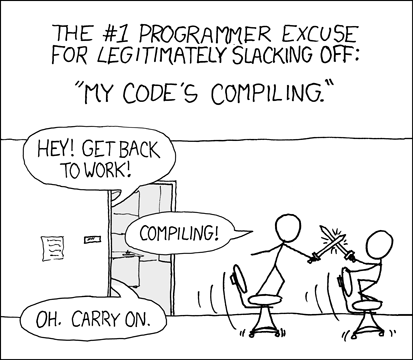
\includegraphics[width=0.5\textwidth,height=\textheight]{"images/codecomic2.png"}
\end{frame}

\begin{frame}[fragile]{There is no Santa Claus: AGG (2006)}
\protect\hypertarget{there-is-no-santa-claus-agg-2006-6}{}
\tiny

\begin{Shaded}
\begin{Highlighting}[]
\KeywordTok{stargazer}\NormalTok{(regols2,regexp2, }\DataTypeTok{type=}\StringTok{\textquotesingle{}latex\textquotesingle{}}\NormalTok{, }\DataTypeTok{se =} \KeywordTok{list}\NormalTok{(regols2}\OperatorTok{$}\NormalTok{rse,regexp2}\OperatorTok{$}\NormalTok{rse),}
          \DataTypeTok{header=}\OtherTok{FALSE}\NormalTok{,  }\DataTypeTok{title=}\StringTok{"AGG replication 2"}\NormalTok{,}\DataTypeTok{omit.stat=}\KeywordTok{c}\NormalTok{(}\StringTok{"f"}\NormalTok{, }\StringTok{"ser"}\NormalTok{), }\DataTypeTok{single.row =} \OtherTok{TRUE}\NormalTok{)}
\end{Highlighting}
\end{Shaded}

\begin{table}[!htbp] \centering 
  \caption{AGG replication 2} 
  \label{} 
\begin{tabular}{@{\extracolsep{5pt}}lcc} 
\\[-1.8ex]\hline 
\hline \\[-1.8ex] 
 & \multicolumn{2}{c}{\textit{Dependent variable:}} \\ 
\cline{2-3} 
\\[-1.8ex] & \multicolumn{2}{c}{vote02} \\ 
\\[-1.8ex] & (1) & (2)\\ 
\hline \\[-1.8ex] 
 contact & 2.688$^{***}$ (0.260) &  \\ 
  state & 2.364$^{*}$ (1.296) & 2.632$^{**}$ (1.296) \\ 
  comp\_mi & $-$1.793$^{***}$ (0.305) & $-$1.769$^{***}$ (0.305) \\ 
  comp\_ia & $-$0.566 (0.685) & $-$0.667 (0.686) \\ 
  persons & 7.001$^{***}$ (0.064) & 7.005$^{***}$ (0.064) \\ 
  age & 0.346$^{***}$ (0.002) & 0.346$^{***}$ (0.002) \\ 
  female2 & $-$1.174$^{***}$ (0.062) & $-$1.173$^{***}$ (0.062) \\ 
  newreg & 5.456$^{***}$ (0.111) & 5.458$^{***}$ (0.111) \\ 
  vote00 & 37.090$^{***}$ (0.074) & 37.092$^{***}$ (0.074) \\ 
  vote98 & 21.657$^{***}$ (0.082) & 21.659$^{***}$ (0.082) \\ 
  fem\_miss & $-$32.082$^{***}$ (0.241) & $-$32.113$^{***}$ (0.241) \\ 
  `contact(fit)` &  & 0.513 (0.420) \\ 
 \hline \\[-1.8ex] 
Observations & 1,905,320 & 1,905,320 \\ 
R$^{2}$ & 0.288 & 0.288 \\ 
Adjusted R$^{2}$ & 0.288 & 0.288 \\ 
\hline 
\hline \\[-1.8ex] 
\textit{Note:}  & \multicolumn{2}{r}{$^{*}$p$<$0.1; $^{**}$p$<$0.05; $^{***}$p$<$0.01} \\ 
\end{tabular} 
\end{table}
\end{frame}

\begin{frame}{There is no Santa Claus: AGG (2006)}
\protect\hypertarget{there-is-no-santa-claus-agg-2006-7}{}
Our OLS estimates are still biased. Even with all these controls,
\(\tilde{\tau}>\tau\).

Unless you had a variable that told you if the person is the type to
answer and talk to an unknown caller about voting, the kitchen sink
approach will not solve the OVB problem.
\end{frame}

\end{document}
